% !TeX encoding = UTF-8
% !TeX program = pdflatex
% !TeX spellcheck = en-US

\documentclass[11pt]{article}

\usepackage[english]{babel}
\usepackage{graphicx}
\usepackage{listings}

\title{RopVis Project \\ \bigskip \large Visual Analytics -  Sapienza}
\author{Pietro Borrello - Serena Ferracci}
\date{19/05/18}

\begin{document}

\maketitle

\section{Introduction}
Return-oriented programming (ROP) is an exploiting technique that allows an attacker to execute arbitrary code in a running program without injecting it, but through a chain of redirections in the program memory itself. \cite{rop}

\bigskip
The attack scenario is based on a controlled stack frame, where the return address can be overwritten. This is an advanced version of the ``return to libc attack'' \cite{libc} where multiple pieces of code are called in sequence to provide the needed code semantics execution: the attack combines a large number of short instruction sequences (called \textit{gadgets} from now on) that allow arbitrary computation. This is resilient to mitigation as non executable memory areas.

Each gadget is in the form of a couple of instruction followed by a return. This allows the attacker to place a sequence of gadget addresses on the stack (called \textit{ROPChain}) from the return address on, that will be executed thanks to the semantics of the ret instruction.

\section{The Problem}
There exists automatic tools to find the suitable gadgets to create the final chain, but all of these tools present the attacker with a textual list of all the found gadgets. Then the attacker has to filter that list on the terminal with \texttt{grep} or similar commands. This becomes frustrating and infeasible with the growing of the complexity of the needed chain.

This is an example of the most simple ROPChain to spawn a shell in the libc standard library:

\begin{lstlisting}
rop = ''
rop += p64(0x0000000000402112) # pop rdi; ret;
rop += '/bin/sh\x00'
rop += p64(0x00000000004106ca) # pop rsi; ret;
rop += p64(WRITABLE_ADDRESS)
rop += p64(0x000000000041a247)
        # mov qword ptr [rsi], rdi; ret;
rop += p64(0x0000000000402112) # pop rdi; ret;
rop += p64(WRITABLE_ADDRESS)
rop += p64(0x00000000004106ca) # pop rsi; ret;
rop += p64(0x0)
rop += p64(0x0000000000400d5e) # pop rax; ret;
rop += p64(0x000000000000003b)
rop += p64(0x000000000041b605) # syscall; ret;
\end{lstlisting}

\bigskip
Where \texttt{p64()} transforms an address to the string representation of it in 64 bits, to be able to place it on the stack:
\begin{lstlisting}
>>> p64(0x1122334455667788)
          '\x88\x77\x66\x55\x44\x33\x22\x11'
\end{lstlisting}

The comment near each instruction represents the instructions in that gadget to be executed.

\bigskip
The problem is that it never happens that the gadget are so simple and clear. Mixed with the instruction the attacker needs, there can be register modifications and memory accesses that can ruin the generated semantics, so choosing the next gadget to use is a delicate task. This becomes a pain, as the size of the chain grows and the number of constraints to maintain in mind increases.
Moreover the number of gadget available in a binary is huge (from 1.500 for a middle sized binary to more than 15.000 for a standard library) so naively searching for useful and correct gadgets between them is impossible.

 Automatic tools that generate the chain exist but usually they fail and leave the attacker alone. So there is a lack of an effective tool to help developing the exploit.

\section{Proposed Solution}

We propose to apply Visual Analytics methods to the problem. The aim is to develop an interface that will help the construction of the chain for the exploit.
The binary that will be the source of the gadgets is analyzed by the backend server that produces a list of semantically meaningful gadgets. This means that only gadgets that have a clear effect are maintained.

The interface will contain the list of all meaningful gadget, divided by class, and by effects on parameters, in which the user can make queries on the desired features and immediately visualize the gadgets that satisfy them.
Queries may involve searching for gadgets that have a particular semantical meaning, but for example, don't modify some registers that have yet been set or access the memory only by some controlled registers, not to crash the program.

Clicking on a gadget will show its features (that will be encoded with additional visual hints). Each class of gadget has a set of attributes:

\bigskip

\begin{center}
  \begin{tabular}{|l|l|}
    \hline
    \textbf{Gadget} & \\ \hline
    type & the class of the gadget \\ \hline
    params & the parameters of the gadget \\ \hline
    hex & the x86 bytes instructions in the gadgets \\ \hline
    disasm & the x86 disassembled instructions \\ \hline
    address & the address where the gadget starts in memory \\ \hline
    address\_end & the address where the gadget ends in memory \\ \hline
    modified\_regs & the registers modified by the execution of the gadget \\ \hline
    mem & the registers that the gadget uses to access memory \\ \hline
    stack\_fix & the delta in the stack after the gadget execution \\ \hline
    retn & how many words the ret instruction at the end pops out \\ \hline
  \end{tabular}
\end{center}

\bigskip
Each gadget has a specific type, between:

\bigskip\noindent
\texttt{LoadConst, SetZero, IncReg, CopyReg,  BinOp, ReadMem, WriteMem,}

\noindent\texttt{OpEsp, Lahf, ReadMemOp, WriteMemOp}

\bigskip
The gadgets in the main view are hierarchically ordered by class, and then by parameters. The size of each node in the main view encodes the number of gadgets of that class, to quickly give an hint on the overall view.

\bigskip
Once clicked on a gadget the user can add it to the chain view in which is displayed the ROPChain that is building. This will trigger the recomputation for the registers the user has successfully set with the chain, and by default the view of the whole gadgets will display only the gadgets safe with respect to modified registers, that the user can choose.

Inside a gadget class the user can additionally trigger a cluster view, in which similar gadgets are displayed near each other to be able to quickly discriminate the possibilities from which it has to chose.

An example of a prototyping interface is:

\begin{center}
  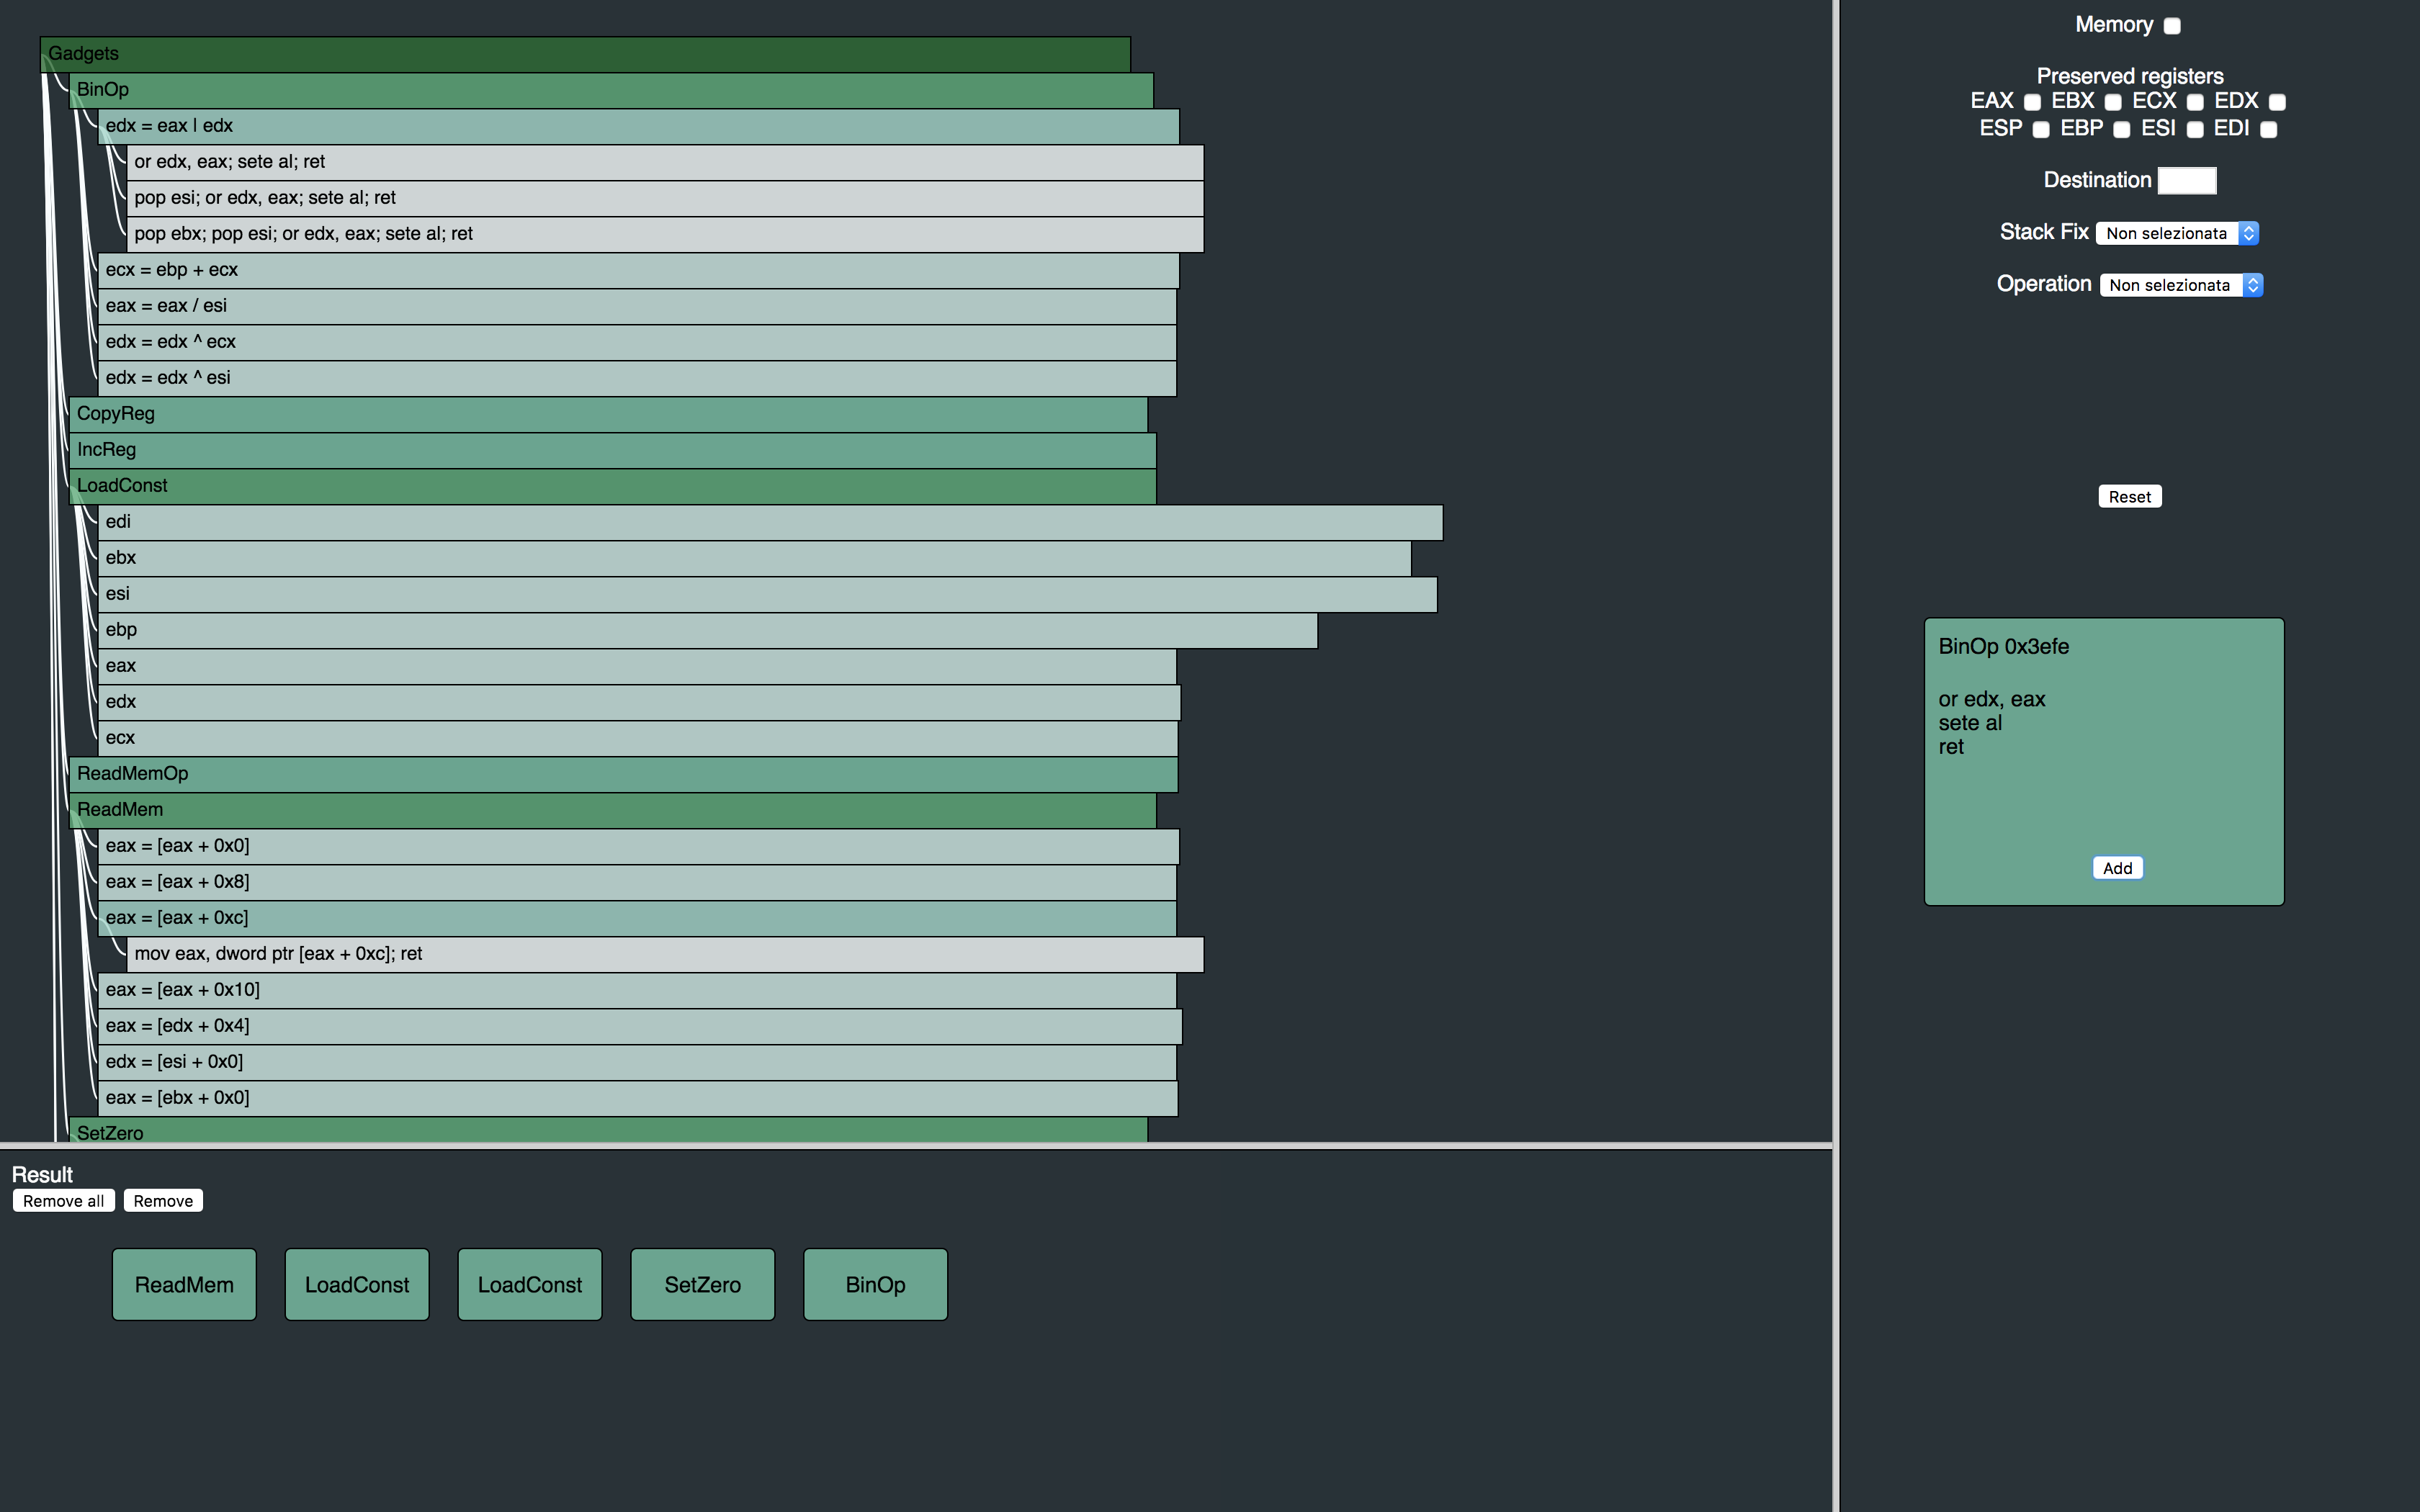
\includegraphics[width=0.9\textwidth]{ropvis-prototype}
\end{center}




\begin{thebibliography}{99}
  \bibitem{rop}
    Hovav Shacham,
    The Geometry of Innocent Flesh on the Bone: Return-into-libc without Function Calls (on the x86),
    CCS,
    2007.
  \bibitem{libc}
    Nergal,
    The advanced return-into-lib(c) exploits (PaX case study),
    Phrack Magazine 58(4),
    Dec. 2001.

\end{thebibliography}

\end{document}
